\title{Parametric RSA applied to Mixed-Gambles Task}
\author{Charles Zheng, Sanmi Koyejo and Russ Poldrack}
\date{\today}

\documentclass[12pt]{article} 

% packages with special commands
\usepackage{amssymb, amsmath}
\usepackage{epsfig}
\usepackage{array}
\usepackage{ifthen}
\usepackage{color}
\usepackage{fancyhdr}
\usepackage{graphicx}
\usepackage{mathtools}
\usepackage{csquotes}
\definecolor{grey}{rgb}{0.5,0.5,0.5}

\begin{document}
\maketitle

\newcommand{\tr}{\text{tr}}
\newcommand{\E}{\textbf{E}}
\newcommand{\diag}{\text{diag}}
\newcommand{\argmax}{\text{argmax}}
\newcommand{\Cov}{\text{Cov}}
\newcommand{\Var}{\text{Var}}
\newcommand{\argmin}{\text{argmin}}
\newcommand{\Vol}{\text{Vol}}
\newcommand{\comm}[1]{}

\newcommand{\bx}{\boldsymbol{x}}
\newcommand{\by}{\boldsymbol{y}}
\newcommand{\bX}{\boldsymbol{X}}
\newcommand{\bY}{\boldsymbol{Y}}


\section{Introduction}

Representational similarity analysis (Kriegeskorte et al.) is a distance-based approach
for comparing how different subjects or different parts of the brain
differ in perceiving a given fMRI task.
Let $i = 1,\hdots, k$ index a collection of tasks,
and let $r = 1,\hdots, n$ index a set of \emph{representators} to be compared.
A representator could be:
\begin{itemize}
\item The whole brain of a subject.
\item A region of a subject's brain.
\item A model-based prediction of the activity of a brain or region of interest.
\item The subject's behaviorial response to the task (e.g. responses to survey questions)
\item A manual labelling of the task into categories.
\end{itemize}

Each representor produces a representation of each stimulus, denoted $\vec{y}^{(i, r)}$.
The representation could be categorical, scalar-valued or multidimensional,
or even non-numerical, e.g. text descriptions.
Furthermore, the different representors could produce representations of different types.
What is essential to the approach is a way to compute distances between representations coming
from the same representor, giving a $k \times k$ distance matrix
\[
D_{ij}^{(r)} = d^{(r)}(\vec{y}^{(i, r)}, \vec{y}^{(j, r)}).
\]
of pairwise distances between stimuli, for $r = 1,\hdots, n$.
Representational similarity analysis works by comparing these $n$ distance matrices
in order to draw conclusions about the nature of the representors.

Suppose that the representators all produce real, vector-valued representations, of possibly differing dimensionality $v_r$.  Furthermore, suppose we choose a scaled, squared Euclidean distance
\[
d^{(r)}(\vec{a},\vec{b}) = \frac{1}{v_r} ||\vec{a} - \vec{b}||^2.
\]
Here we divide by $v_r$ so that in the commonly encountered case where the representation is obtained by
sampling from a continuous function, the resulting distance is robust to fineness of discretization.

In many experimental designs, we have a parameterization of the stimuli, given by $p \times 1$ a vector $\vec{x}_i$.
We can obtain further insights if we incorporate this knowledge into our representational similarity analysis.

Let us assume that $\vec{y}^{(r)}$ is obtained from a linear mapping from $\vec{x}_i$:
\[
\vec{y}^{(r)} = (B^{(r)})^T \vec{x}_i  + \vec{\mu}^{(r)}
\]
where $B^{(r)}$ is a $p \times v_r$ coefficient matrix.
Then it follows that the distance between stimulus $i$ and $j$ is a function of the difference $\vec{x}_i-\vec{x}_j$, given by
\begin{align*}
D^{(r)}_{ij} &= \frac{1}{v_r} (\vec{y}_i - \vec{y}_j)^T( \vec{y}_i - \vec{y}_j) 
\\&= \frac{1}{v_r} ((B^{(r)})^T\vec{x}_i - (B^{(r)})^T\vec{x}_j)^T((B^{(r)})^T \vec{x}_i - (B^{(r)})^T\vec{x}_j) 
\\&= \frac{1}{v_r} (\vec{x}_i - \vec{x}_j)^T M^{(r)} (\vec{x}_i-\vec{x}_j).
\end{align*}
where $M^{(r)} = B^{(r)} (B^{(r)})^T$.
While $D^{(r)}$ is a $k \times k$ matrix,
$M^{(r)}$ is a $p \times p$ matrix, and hence a much smaller matrix in the common case when
the dimensionality of the stimulus space is lower than the number of stimuli used in the experiment.
We call $M^{(r)}$ the \emph{feature-distance matrix}, since under the linear modelling assumption,
it contains the information sufficient to construct the distance matrix $D^{(r)}$ from the parameter features $\vec{x}_i$.

We can draw interpretable conclusions by comparing the entries of $M^{(r)}$ across representors.
A large value in the $i$th diagonal element of $M^{(r)}$ means that the particular representor is sensitive to the $i$th feature.  Hence on can test the hypothesis that $M^{(r)}_{ii} > M^{(r')}_{ii}$ to conclude that representor $r$ is more sensitive to the $i$th feature than representor $r'$, for instance.

\section{Data}

We used the mixed-gambles data from Tom et al. 2007.
The data consisted of 3 runs for each of 16 subjects.
In each run, 16 different gambling tasks were presented.
These tasks varied in the gain amount and loss amount.

Clusters were obtained using a parametric map from {\tt http://neurovault.org/images/10680/},
then applying thresholding using FSL.
A size threshold was applied, yielding 28 regions of interest.

\begin{figure}[h]
\centering
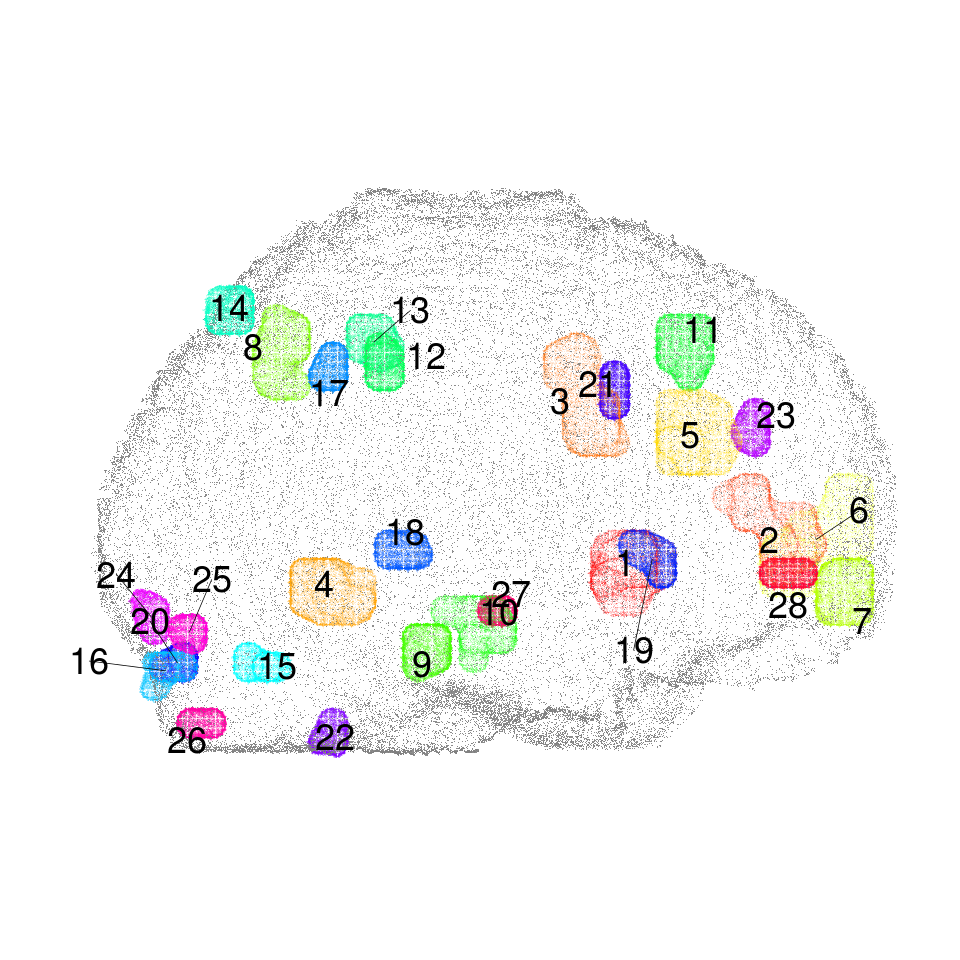
\includegraphics[scale = 0.12]{../a7plots/all_rois_view1.png}
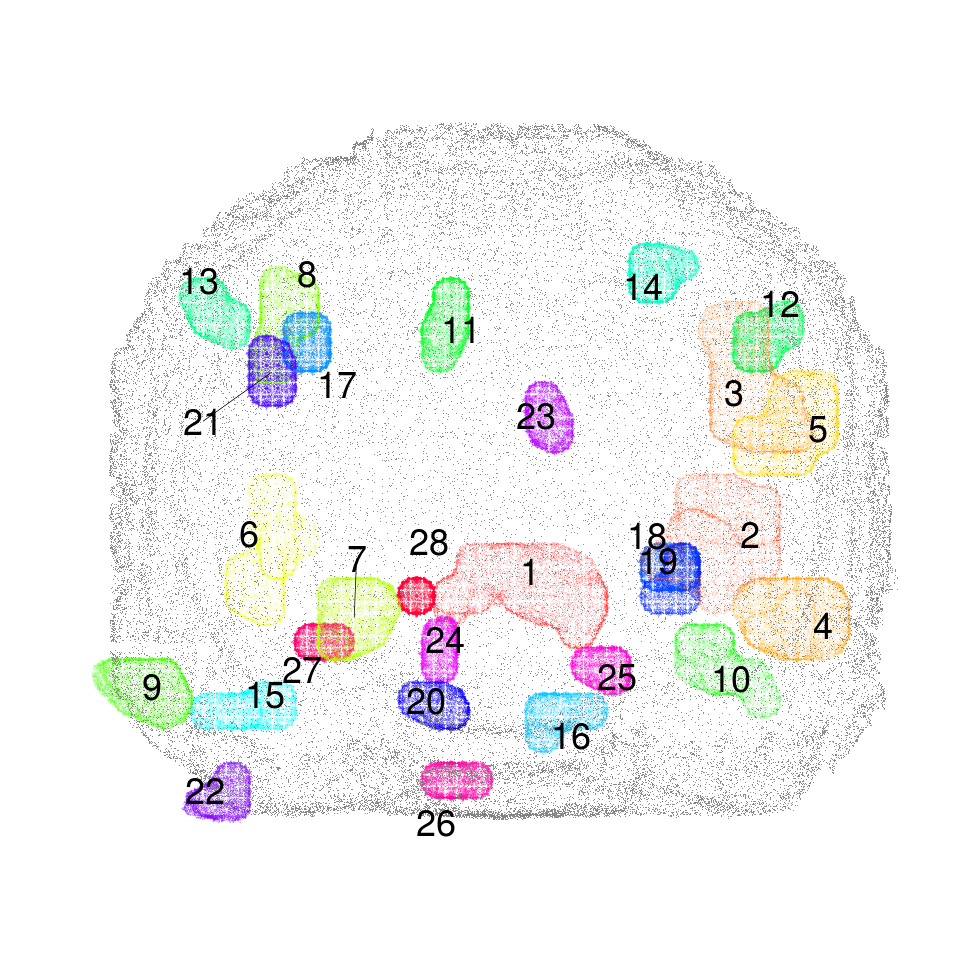
\includegraphics[scale = 0.12]{../a7plots/all_rois_view2.png}
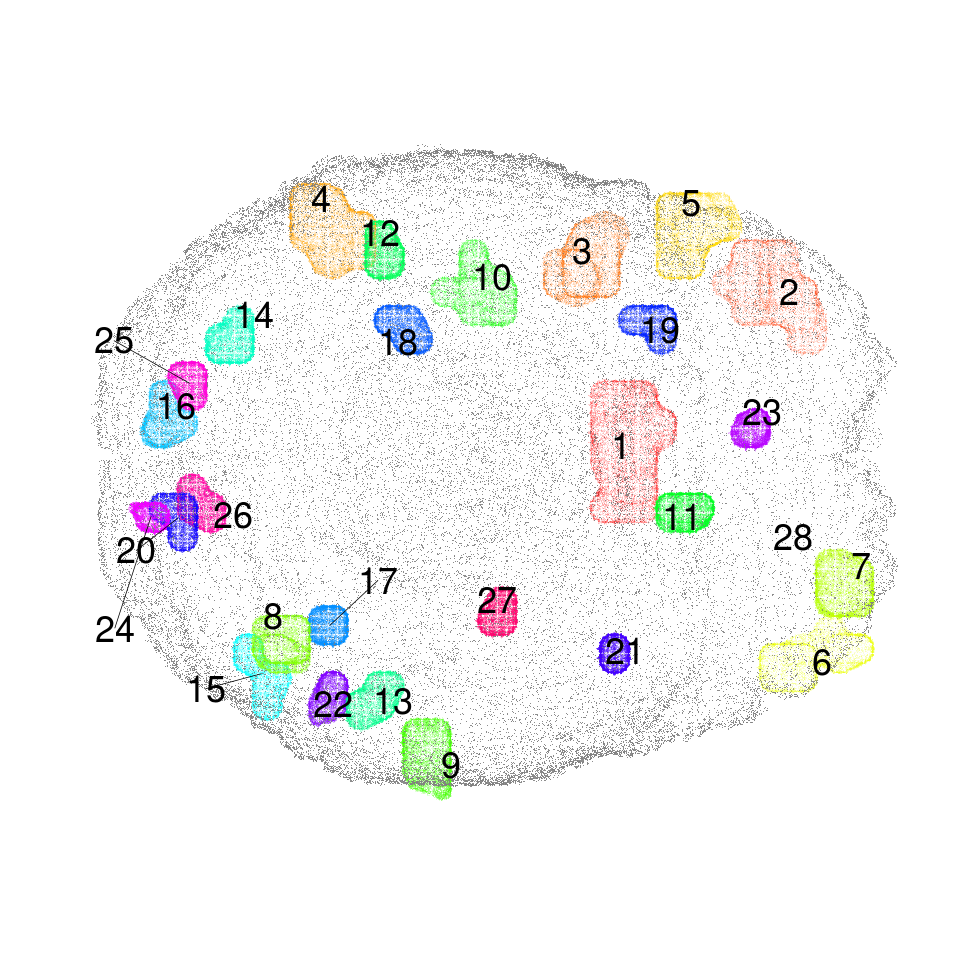
\includegraphics[scale = 0.12]{../a7plots/all_rois_view3.png}
\caption{The 28 regions of interest extracted via thresholding.}
\end{figure}

The scans were registered to a common template, then a standard linear model-based approach
was used to extract an activity level per voxel per event per run.
We extracted the regions of interest from the data.  For a given region of interest, the data takes the form:

\begin{tabular}{|c|c|c|c||c|c|c|c|}
\hline
subject & run & gain & loss & voxel 1 & voxel 2 & ... & voxel $N$ \\
\hline
 1 & 1 & 13 &  6.5 & -222.8994 &  -373.85025 & ... & 12.038\\
... & ... & ... & ... & ... & ... & ... & ...\\
16 & 3 & 37 & 18.5 & -136.89 & -73.49 & ... & 75.068146 \\
\hline
\end{tabular}

where $N$ is the number of voxels in the ROI.

\section{Methods}

We model the data using the following linear model.
Let $s = 1,\hdots, 16$ index the subjects, and $e = 1,\hdots, 48$ index the events from all runs combined.
Let $r = 1,\hdots, 28$ index the regions of interest, and $m = 1,\hdots, v_r$ the voxels in the ROI.
Then the model for the activity of the $m$th voxel in the $r$th roi is
\[
y_{s, e, r, m} = \langle \vec{x}_{e}, \beta_{s, r, m} \rangle + \mu_{s, r, m} + \epsilon_{s, e, r, m}
\] 
where $y_{s, e, r, m}$ is the activity of the $m$th voxel for the $s$th subject in the $e$th event (a scalar quantity),
$\vec{x}_e$ is the 2x1 vector of parameters (gain and loss) for the $e$th event ,
and $\beta_{s, r, m}$ is a vector of coefficients specific to the subject and to the voxel.
The coefficient vector $\beta_{s, r, m}$ is viewed as a \emph{random effect} such to variation between subjects.
$\mu_{s, r, m}$ is a subject-specific mean term for the voxel.
Meanwhile, assume that the noise term $\epsilon_{s, e, r, m}$ is normal $N(0, \sigma^2_{s, r, m})$
with zero mean, and covariance specific to the subject and voxel.
Assume that the noise terms for are correlated \emph{within an event} but are independent \emph{across events}.  This assumption may not be realistic, since there is usually some autocorrelation across events.
\[
\text{ if }e \neq e' \text{ or }s \neq s', \text{ then }\Cov(e_{s, e, r, m}, e_{s', e', r, m}) = 0 .
\]
\[
\Cov(e_{s, e, r, m}, e_{s, e, r', m'}) = \sigma_{r,m,r',m'}.
\]
Write $\Sigma_{r}$ for the $n_v \times n_v$ covariance matrix for voxels within a region of interest.

The parametric RSA approach is to define for each subject and ROI the feature-distance matrix $M^{(s, r)}$ with entries
\[
M^{(s, r)}_{ij} = \frac{1}{v_r}\langle \beta_{s, r, i}, \beta_{s, r, j }\rangle.
\]
The randomness of $\beta_{s, r, m}$ induces a random distribution for $M^{(s, r)}$ for a given randomly sampled subject. Let $F^{(r)}$ denote the distribution of the $2 \times 2$ matrix $M^{(s, r)}$.

\subsection{Estimation}

We develop new methodology to estimate the matrices $M^{(s, r)}$.
The ``naive'' approach would be to obtain an estimate of the coefficient matrix, $\hat{B}^{(s, r)}$, then set
\[
\hat{M}_{naive}^{(s, r)} = \hat{B}^{(s, r)} (\hat{B}^{(s, r)})^T.
\]
While $\hat{M}_{naive}$ is consistent in the large-sample limit, it is highly biased in finite samples.
Under the assumption that
\[
\vec{y}^{(s, e, r)} = (B^{(s, r)})^T \vec{x}_{e} + \epsilon^{(r)}
\]
where $\epsilon^{(r)}$ has mean $0$ and covariance $\Sigma^{(r)}$,
and under the condition that the number of events is larger than the number of features,
it follows that the OLS estimate 
\[
\hat{B}^{(s, r)} = (X^T X)^{-1}X^T Y^{s, r}
\]
has mean $B^{(s, r)}$ and covariance given by
\[
\Cov(\hat{B}^{(s, r)}_{ij}, \hat{B}^{(s, r)}_{kl}) = ((X^TX)^{-1})_{ik} \Sigma^{(r)}_{jl}.
\]
It then follows that
\[
\E[\hat{M}_{naive}^{(s, r)}] = M^{(s, r)} + (X^T X)^{-1} \tr(\Sigma^{(r)}).
\]
The term $(X^T X)^{-1}$ is of order $O(1/n_e)$, where $n_e$ is the number of events per subject,
hence the bias in $\hat{M}_{naive}$ is severe in designs with few events per subject.
We can obtain an improved estimator simply by correcting the bias, defining
\[
\hat{M} = \hat{M}_{naive} - (X^T X)^{-1} \tr(\hat{\Sigma}^{(r)}),
\]
where $\hat{\Sigma}^{(r)}$ is an unbiased estimate of $\Sigma^{(r)}$.

\subsection{Testing}

We are interested in comparing feature-distance matrices across regions of interest.
Suppose we wish to compare the $ij$th entry of the feature-distance matrix between region $r$ with region $r'$.  The null hypothesis is that
\[
H_0: \E[M^{(s, r)}_{ij}] = \E[M^{(s, r')}_{ij}]
\]
where the expectation is taken across the distribution of subjects.
Since $\hat{M}^{(s, r)}$ is an unbiased estimate of $M^{(s, r)}$, the null hypothesis $H_0$ is equivalent to the hypothesis
\[
H_0': \E[\hat{M}^{(s, r)}_{ij}] = \E[\hat{M}^{(s, r')}_{ij}].
\]
Testing of $H_0'$ is accomplished by first estimating $\hat{M}^{(s, r)}$ and $\hat{M}^{(s, r')}$ for subjects $s = 1,\hdots, 16$,
then applying a paired, separate-variance
two-sample t-test to the paired data $\{(\hat{M}^{(s, r)}_{ij}, \hat{M}^{(s, r')}_{ij})\}_{s=1}^{16}$.

We carry out the testing procedure for every entry in $M$ and every pair of distinct regions of interest.
In a confimatory study, we would then have to apply multiple testing correction in order to assess significance.
However, as an exploratory step, we simply present the results marginally.

\section{Results}

First, we summarize the results for each of the three distinct entries of $M_{ij}$.
For each entry $ij$, there are 28 choose 2 = 378 tests of comparison between ROIs.
Hence, at the 0.05 significance level, we expect an average of 18.9 rejections under the global null hypothesis (that all ROIs are equivalent).
We get the following results:

\begin{figure}[h]
\begin{tabular}{c|c}
$(i, j)$ & no. rejections at $\alpha = 0.05$\\\hline
$(1, 1)$ & 31\\
$(1,2)$ & 31\\
$(2,2)$ & 11\\
\end{tabular}
\end{figure}

While the total number of rejections for $M_{(2,2)}$ (the term corresponding to loss sensitivity)
is less than chance, some of those rejections may be informative when we consider
pairs of ROIs which were rejected for multiple entries of $M$. 

The overlaps in rejections are displayed in figure 2.
\begin{figure}[h]
\centering
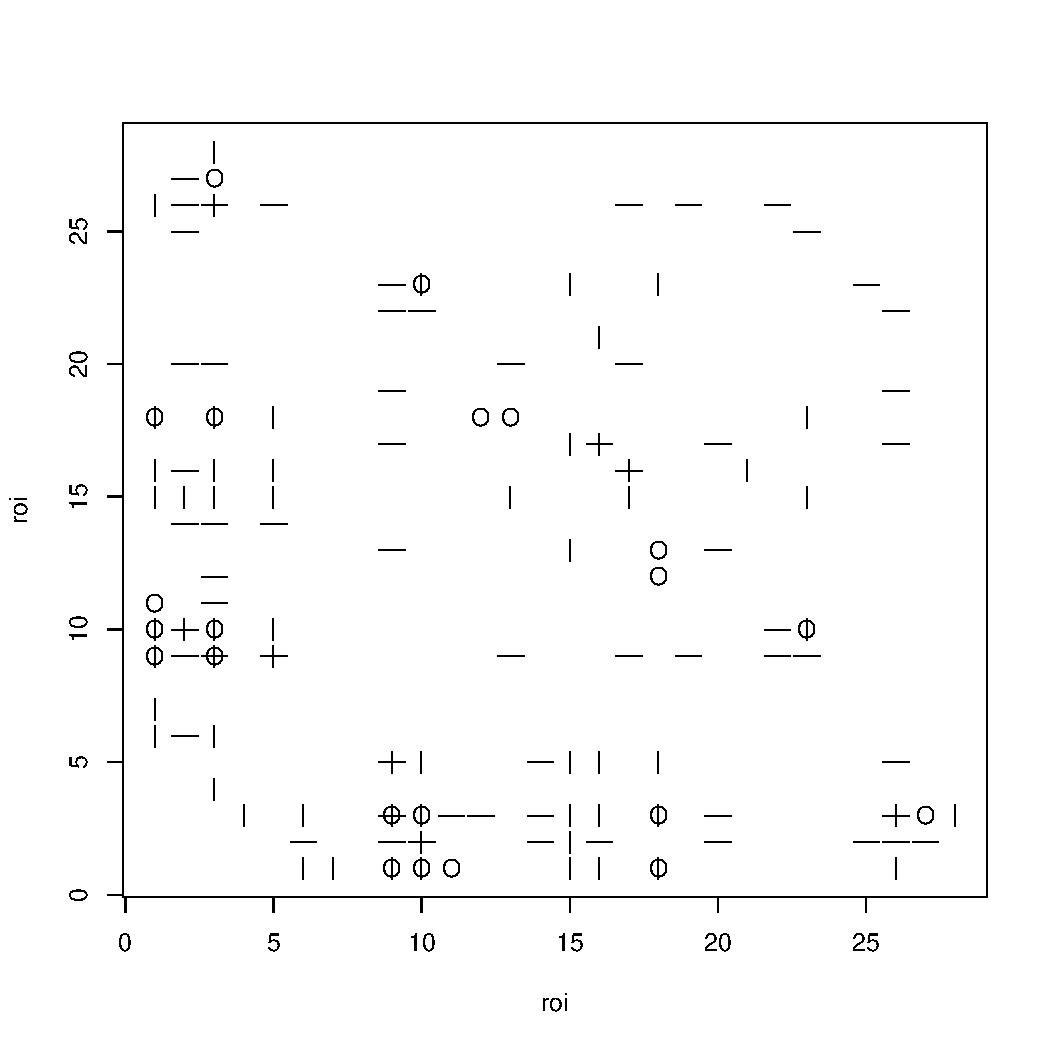
\includegraphics[scale = 0.5]{../a7plots/rejs.pdf}
\caption{Rejections of null hypothesis for pairs of ROIs. -- = rejected for $M_{1,1}$, $|$ = rejected for $M_{2,2}$, and O indicates rejected for $M_{2,2}$}
\end{figure}

In figures 4+, we single out some regions of interest which had particularly large numbers of rejections.

\begin{figure}[h]
\centering
\begin{tabular}{ccc}
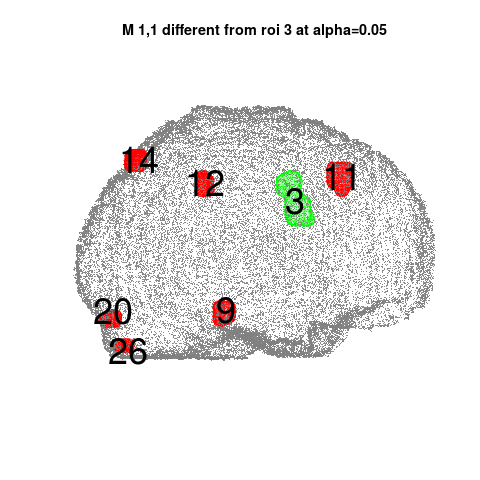
\includegraphics[scale = 0.24]{../a7plots/d_1r_3_view1.png} & 
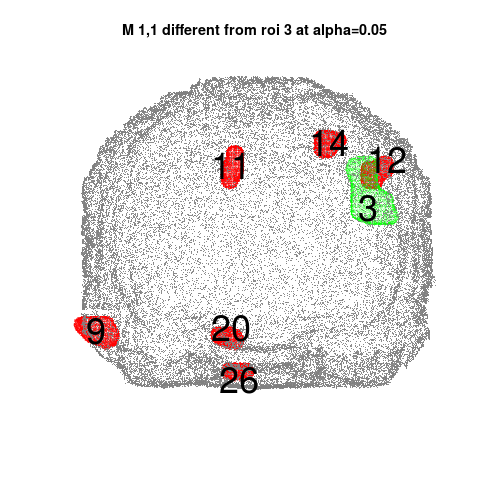
\includegraphics[scale = 0.24]{../a7plots/d_1r_3_view2.png} & 
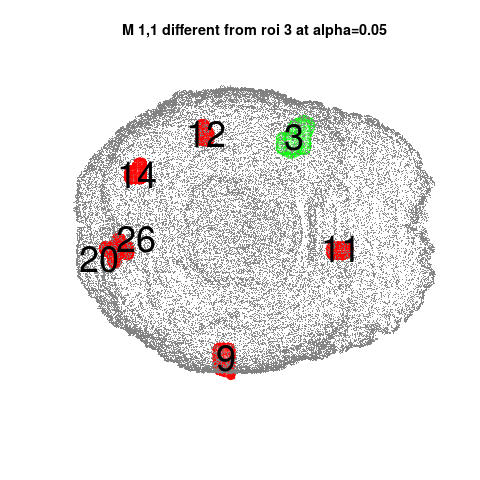
\includegraphics[scale = 0.24]{../a7plots/d_1r_3_view3.png} \\ 
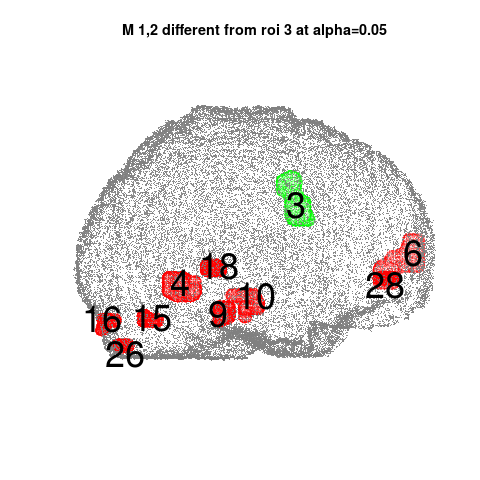
\includegraphics[scale = 0.24]{../a7plots/d_2r_3_view1.png} & 
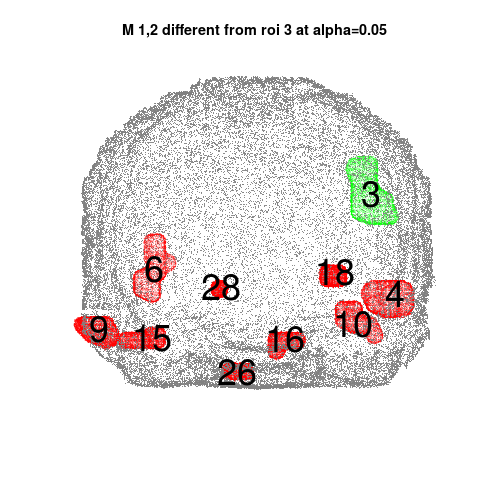
\includegraphics[scale = 0.24]{../a7plots/d_2r_3_view2.png} & 
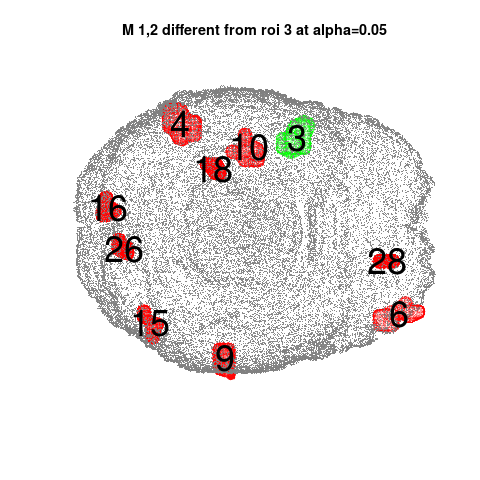
\includegraphics[scale = 0.24]{../a7plots/d_2r_3_view3.png} \\ 
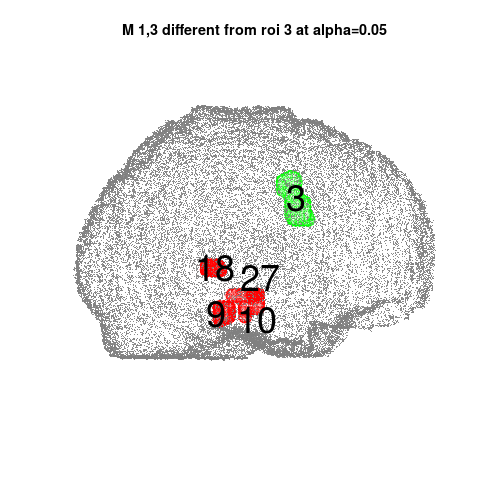
\includegraphics[scale = 0.24]{../a7plots/d_3r_3_view1.png} & 
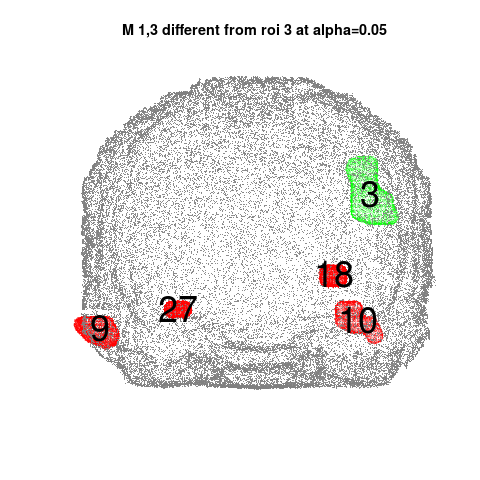
\includegraphics[scale = 0.24]{../a7plots/d_3r_3_view2.png} & 
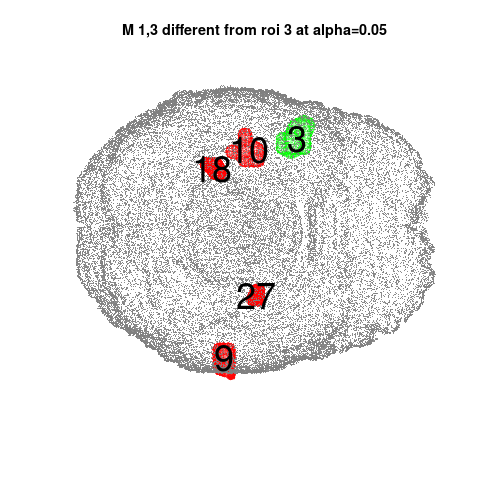
\includegraphics[scale = 0.24]{../a7plots/d_3r_3_view3.png} \\ 
\end{tabular}
\caption{ROI 3 (19 rejections)}
\end{figure}

\begin{figure}[h]
\centering
\begin{tabular}{ccc}
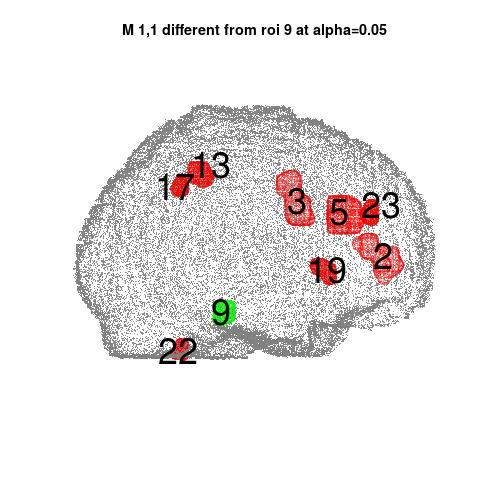
\includegraphics[scale = 0.24]{../a7plots/d_1r_9_view1.png} & 
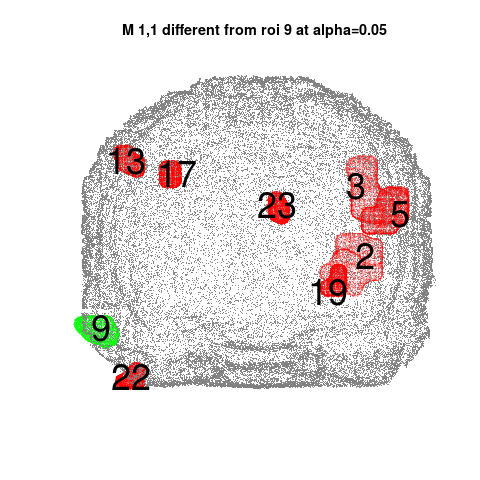
\includegraphics[scale = 0.24]{../a7plots/d_1r_9_view2.png} & 
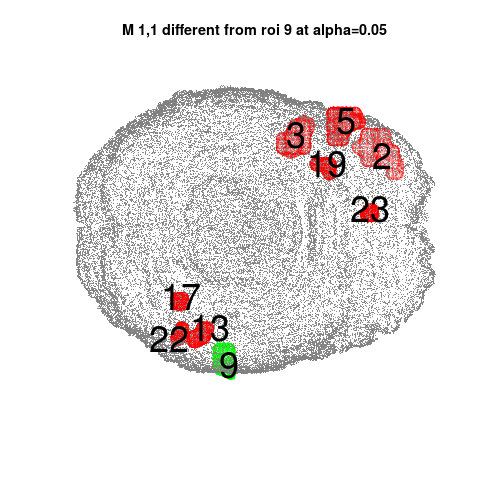
\includegraphics[scale = 0.24]{../a7plots/d_1r_9_view3.png} \\ 
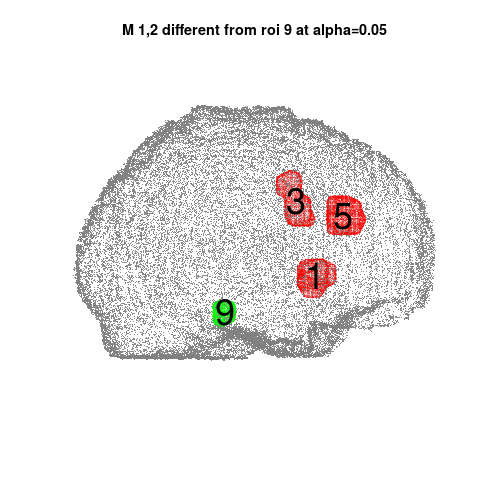
\includegraphics[scale = 0.24]{../a7plots/d_2r_9_view1.png} & 
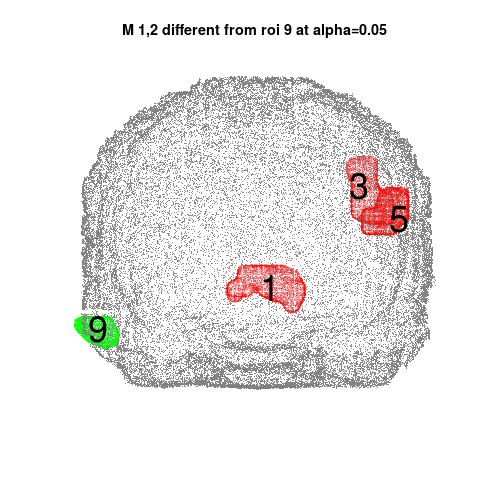
\includegraphics[scale = 0.24]{../a7plots/d_2r_9_view2.png} & 
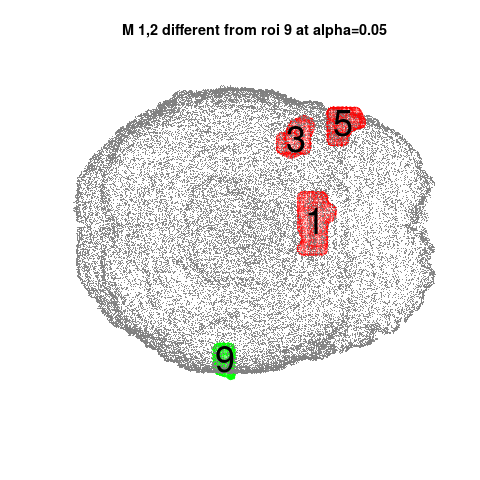
\includegraphics[scale = 0.24]{../a7plots/d_2r_9_view3.png} \\ 
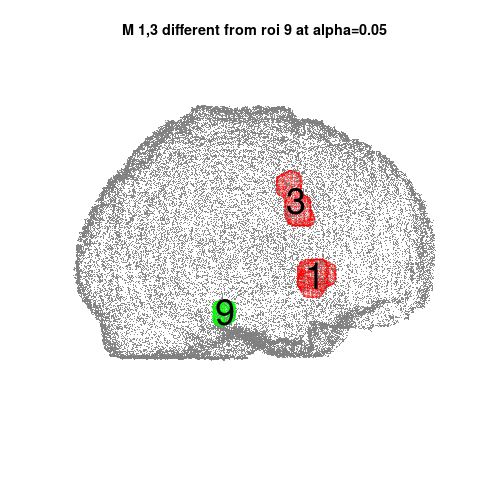
\includegraphics[scale = 0.24]{../a7plots/d_3r_9_view1.png} & 
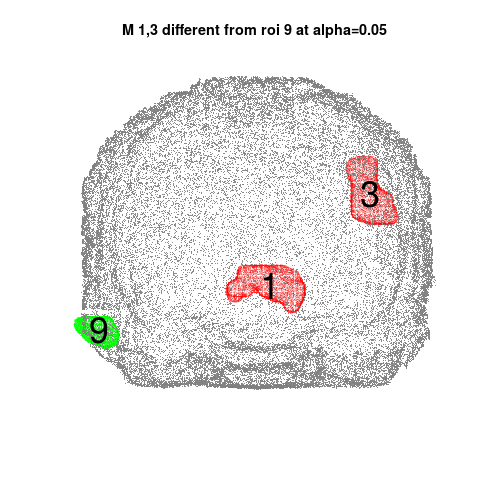
\includegraphics[scale = 0.24]{../a7plots/d_3r_9_view2.png} & 
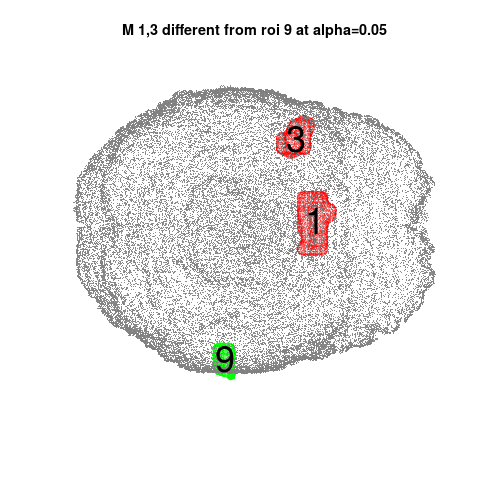
\includegraphics[scale = 0.24]{../a7plots/d_3r_9_view3.png} \\ 
\end{tabular}
\caption{ROI 9 (13 rejections)}
\end{figure}

\begin{figure}[h]
\centering
\begin{tabular}{ccc}
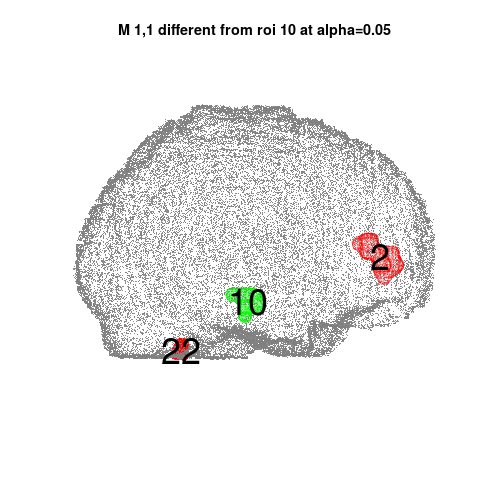
\includegraphics[scale = 0.24]{../a7plots/d_1r_10_view1.png} & 
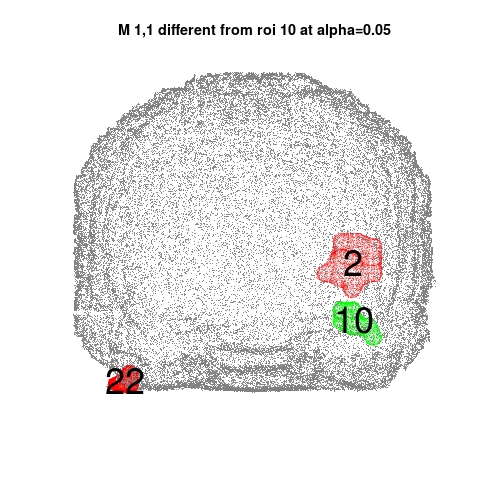
\includegraphics[scale = 0.24]{../a7plots/d_1r_10_view2.png} & 
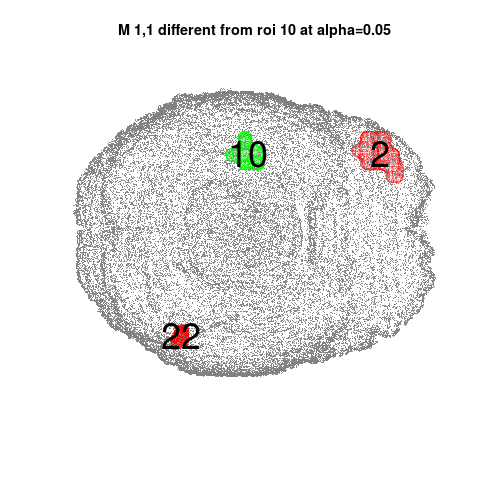
\includegraphics[scale = 0.24]{../a7plots/d_1r_10_view3.png} \\ 
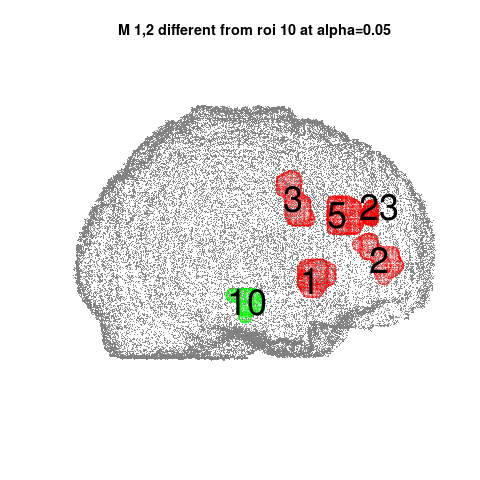
\includegraphics[scale = 0.24]{../a7plots/d_2r_10_view1.png} & 
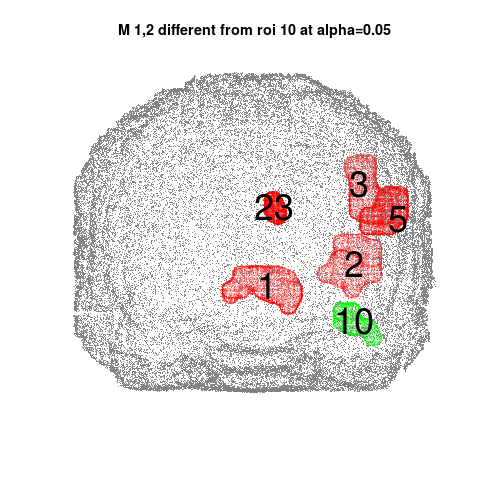
\includegraphics[scale = 0.24]{../a7plots/d_2r_10_view2.png} & 
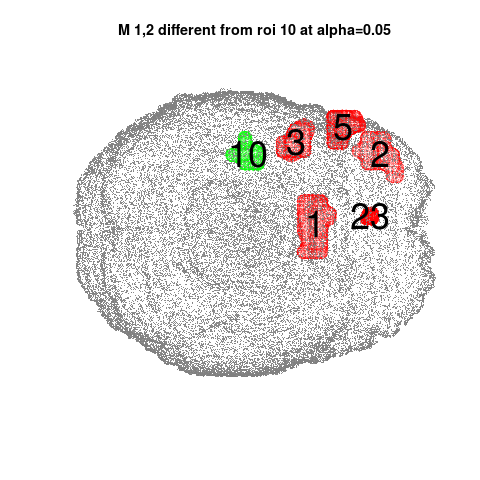
\includegraphics[scale = 0.24]{../a7plots/d_2r_10_view3.png} \\ 
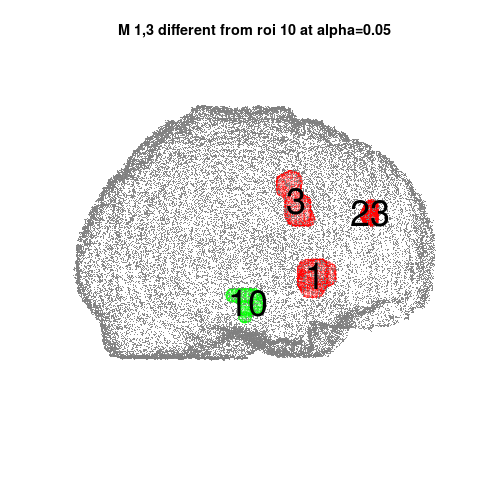
\includegraphics[scale = 0.24]{../a7plots/d_3r_10_view1.png} & 
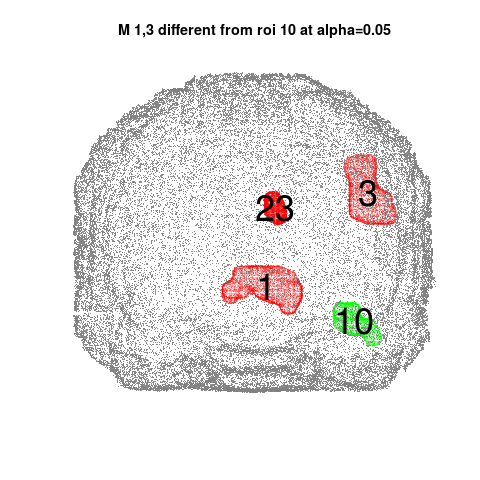
\includegraphics[scale = 0.24]{../a7plots/d_3r_10_view2.png} & 
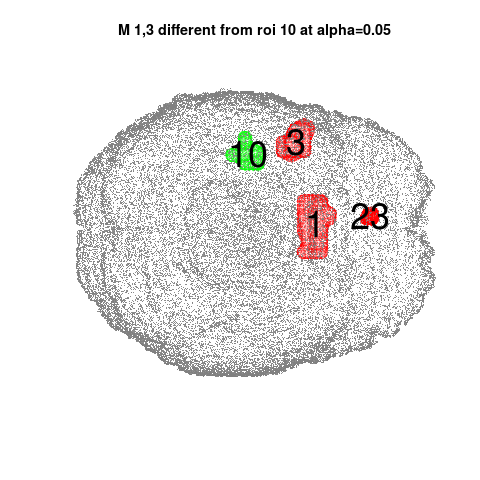
\includegraphics[scale = 0.24]{../a7plots/d_3r_10_view3.png} \\ 
\end{tabular}
\caption{ROI 10 (10 rejections)}
\end{figure}

Other ROIs with more than 10 rejections:

\begin{figure}[h]
\centering
\begin{tabular}{ccc}
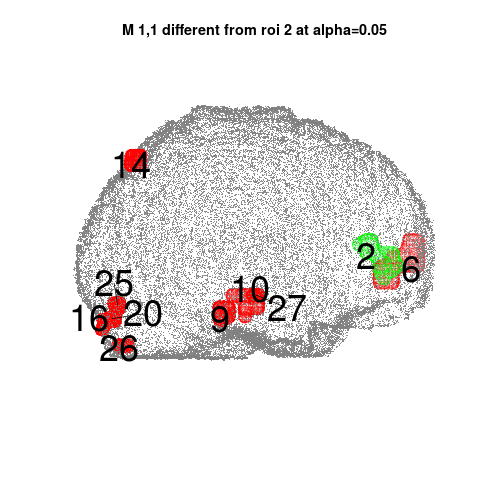
\includegraphics[scale = 0.24]{../a7plots/d_1r_2_view1.png} & 
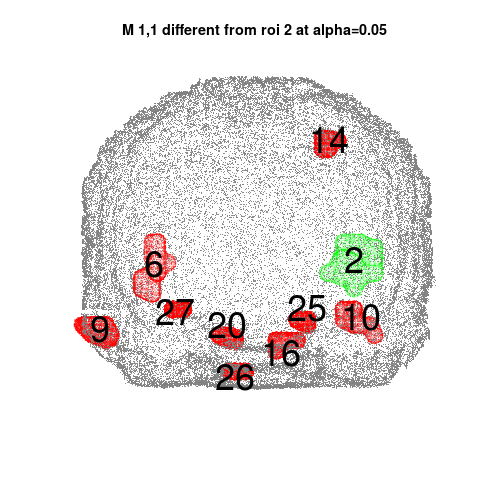
\includegraphics[scale = 0.24]{../a7plots/d_1r_2_view2.png} & 
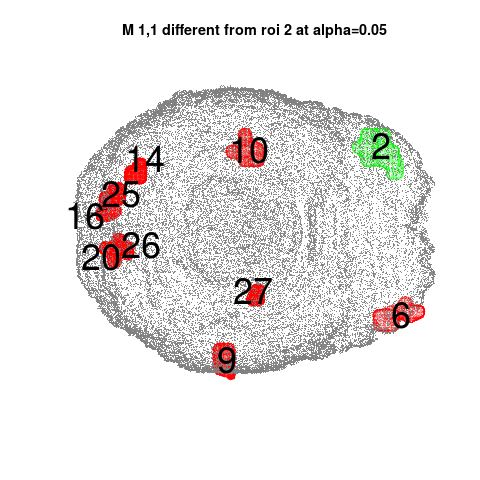
\includegraphics[scale = 0.24]{../a7plots/d_1r_2_view3.png} \\ 
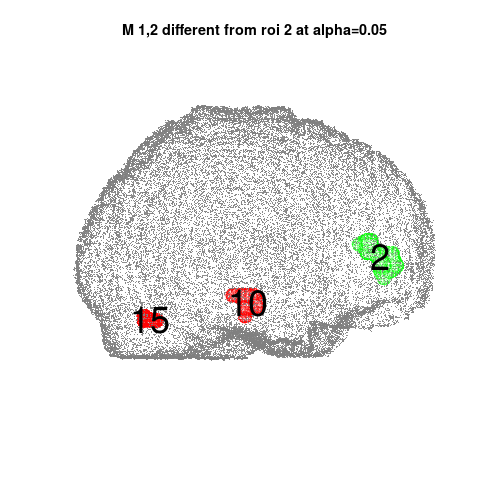
\includegraphics[scale = 0.24]{../a7plots/d_2r_2_view1.png} & 
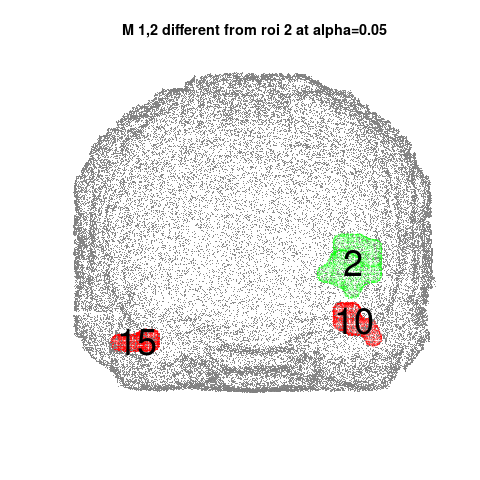
\includegraphics[scale = 0.24]{../a7plots/d_2r_2_view2.png} & 
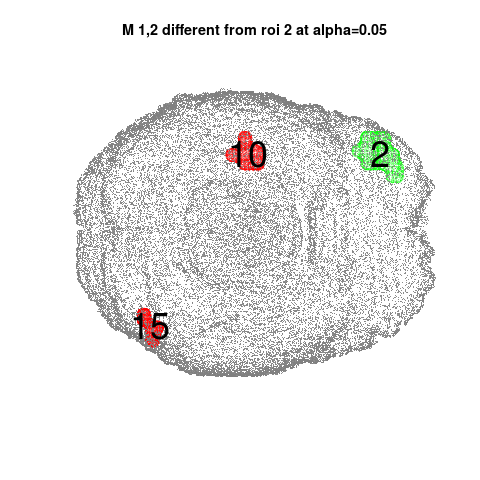
\includegraphics[scale = 0.24]{../a7plots/d_2r_2_view3.png} \\ 
\end{tabular}
\caption{ROI 1 (12 rejections)}
\end{figure}

\begin{figure}[h]
\centering
\begin{tabular}{ccc}
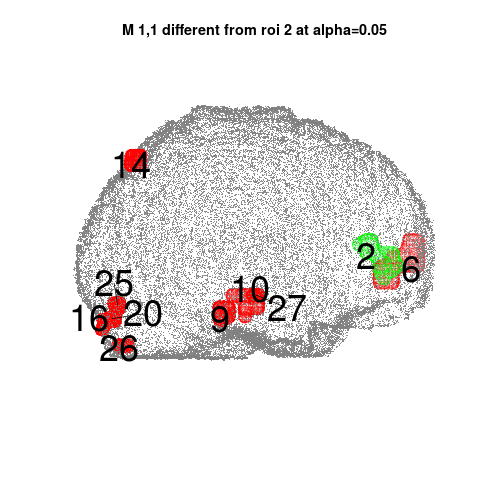
\includegraphics[scale = 0.24]{../a7plots/d_1r_2_view1.png} & 
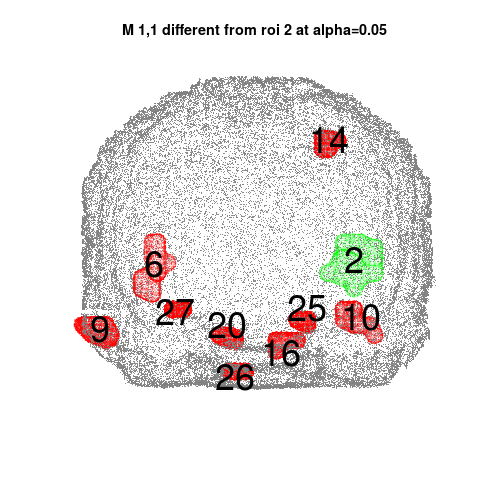
\includegraphics[scale = 0.24]{../a7plots/d_1r_2_view2.png} & 
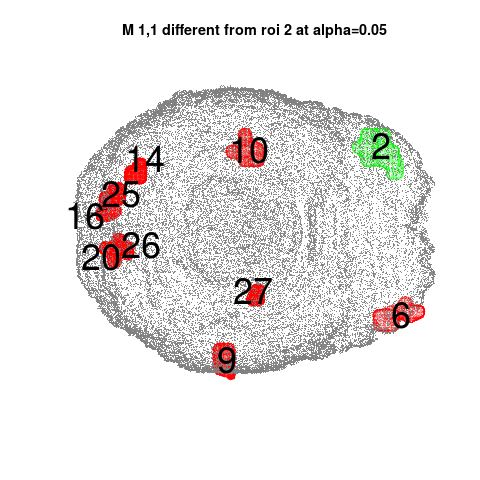
\includegraphics[scale = 0.24]{../a7plots/d_1r_2_view3.png} \\ 
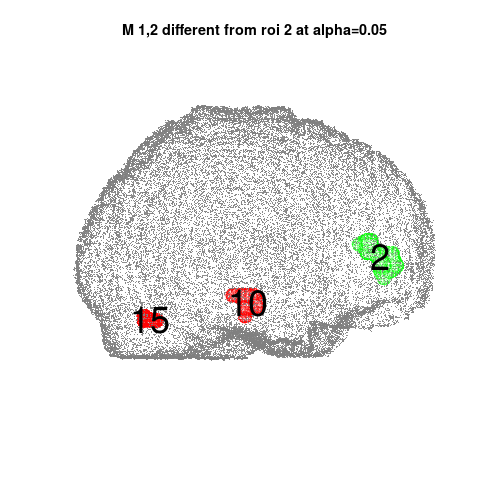
\includegraphics[scale = 0.24]{../a7plots/d_2r_2_view1.png} & 
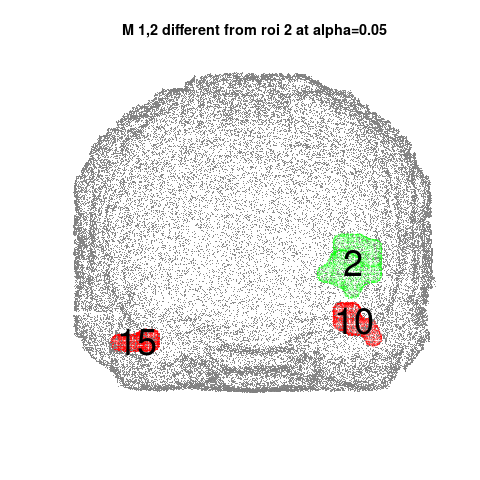
\includegraphics[scale = 0.24]{../a7plots/d_2r_2_view2.png} & 
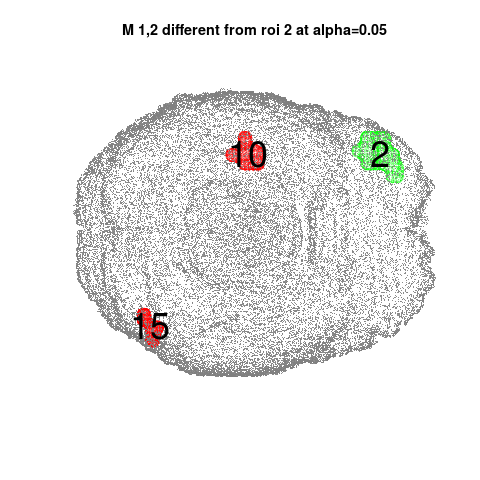
\includegraphics[scale = 0.24]{../a7plots/d_2r_2_view3.png} \\ 
\end{tabular}
\caption{ROI 2 (11 rejections)}
\end{figure}

\end{document}



